% Chapitre de contribution n° 5 (TOP20 pick 5, id ED-17)
% Sources : papers/prog_superfluid_structure_factor/ (main.tex, AUDIT.md, REVISION.md, publication_meta.json,
% gen_numbers.tex, data/he4_Sk_donnelly_table14_1.csv, data/test_he4.csv), TOP20.json.
\chapter[Une règle droite, une esquisse fausse]{Une règle prouvée droite montre que notre propre esquisse était fausse}
\reference{Publié le 26 octobre 2026.\\ doi:10.5281/\\zenodo.23653846}

\section*{L'idée en une image}

\begin{analogie}
Vous démontrez d'abord que votre règle est parfaitement droite. Puis vous la posez sur un dessin que vous aviez fait
vous-même quelques semaines plus tôt, et vous voyez qu'il est tordu. La règle n'est pas en cause ; l'esquisse, si.

\emph{Où l'image s'arrête :} ici, la « règle » prouvée parle d'un modèle idéal de fluide ; c'est la mesure de
l'hélium réel, et non la preuve, qui condamne l'esquisse.
\end{analogie}

\section*{Ce qui a été fait}

À très basse température, l'hélium~4 liquide devient superfluide.
On l'étudie en y envoyant des neutrons ou des rayons X et en mesurant comment ils sont déviés ; on en tire le
\emph{facteur de structure} $S(Q)$, qui dit comment les atomes s'organisent à l'échelle $1/Q$. Un argument classique
relie cette mesure à l'énergie des petites ondes qui parcourent le fluide : à vecteur d'onde $k$, l'énergie la plus
basse est au plus $\hbar^2k^2/(2mS(k))$, où $m$ est la masse d'un atome.

Le travail fait deux choses. D'abord, il écrit et prouve dans Lean le cœur mathématique de cet argument, en posant
explicitement comme hypothèses deux ingrédients physiques (une règle de somme et une symétrie $k\leftrightarrow-k$)
qui, eux, ne sont pas démontrés dans Lean. Ensuite, il teste sur des données publiées une « enveloppe » que le projet
avait proposée plus tôt dans le mois, à partir du modèle idéal de gaz de Bogoliubov : $S(Q)\le B(Q)=\sqrt{Q/2k_*}$,
avec $k_*=2mc/\hbar$ et $c=238{,}3$\,m/s la vitesse du son dans l'hélium, ce qui donne $k_*\approx3{,}004$\,Å$^{-1}$.

\begin{encadre}
\textbf{À faire avec une calculatrice : le sommet de la courbe.} Au point le plus haut du tableau, $Q=2{,}058$\,Å$^{-1}$
et l'on mesure $S=1{,}458$. L'enveloppe vaut $B=\sqrt{2{,}058/6{,}008}=\sqrt{0{,}3426}\approx0{,}585$. La mesure est
$1{,}458/0{,}585\approx2{,}49$ fois plus haute que la limite proposée, et la dépasse de $0{,}87$, bien plus que la
marge de tolérance de $0{,}082$.

\textbf{Le modèle idéal, lui, respecte l'enveloppe.} Dans le gaz de Bogoliubov, $S=k/\sqrt{k_*^2+k^2}$. Pour $k=k_*$,
on obtient $1/\sqrt2\approx0{,}707$, et l'enveloppe vaut $\sqrt{1/2}\approx0{,}707$ : égalité exacte, jamais de
dépassement. C'est le témoin qui doit passer, et il passe.
\end{encadre}

Sur les 99 points du tableau de référence (des mesures aux rayons X et aux neutrons rassemblées dans une compilation
publiée), 29 respectent l'enveloppe, 7 la dépassent de moins que la marge (indécis) et 63 la dépassent nettement
(réfutés). Dans la région dite « du roton », entre $1{,}7$ et $2{,}4$\,Å$^{-1}$, les 21 points sont tous réfutés, par un
facteur de $1{,}62$ à $2{,}49$ (figure~\ref{fig:c05}). La lecture est modeste : l'hélium liquide n'est pas un gaz de
Bogoliubov, ce que les manuels disent déjà. Le même article contient donc un résultat formel positif et un résultat
physique négatif, qui porte sur une proposition du projet lui-même.

\begin{figure}[htbp]
\centering
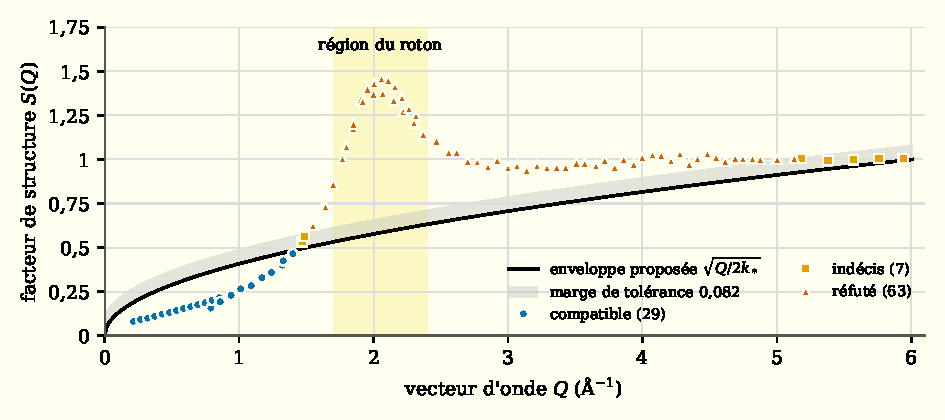
\includegraphics[width=\linewidth]{figures/c05_helium}
\caption{Facteur de structure tabulé de l'hélium~4 (99 points) face à l'enveloppe proposée ; verdicts recalculés avec
la règle de l'article.}
\label{fig:c05}
\end{figure}

\section*{Comment on s'est assuré que ce n'est pas faux}

\niveau{A} \emph{Le juge a regardé}, pour la partie mathématique. Lean, le programme qui contrôle chaque pas d'une
preuve, n'utilise que les trois hypothèses de base admises partout, et le module a été rejoué sans erreur par un
second programme de contrôle le 26 octobre 2026. Deux exemples construits exprès montrent que les hypothèses ne sont
pas décoratives : dans l'un, sans la symétrie, l'étape qui divise par deux devient fausse ($1$ au lieu de $1/2$) ; dans
l'autre, toutes les hypothèses sont vraies à la fois et la borne est atteinte exactement. Un agent d'IA indépendant a
tout recompilé de son côté et y a glissé deux sabotages : une preuve effacée dans un lemme intermédiaire a bien été
signalée, et aussi dans les trois théorèmes principaux qui reposent sur lui ; un axiome caché qui « prouvait » une
absurdité a lui aussi été repéré.

Les données sont \niveau{L} : un tableau publié, mais de seconde main, mesuré entre 1,4 et 4 kelvins et sans barres
d'erreur. Les verdicts sont \niveau{X}. L'auditeur a relu lui-même le tableau brut et retrouvé les mêmes 29, 7 et 63.
Un point est dit honnêtement : la marge de $0{,}082$ (l'écart entre les sommets de deux séries de mesures) a été
fixée \emph{après} avoir vu les données, ce qui s'écarte du plan annoncé. Le résultat du roton n'en dépend pas : sa plus
petite marge, $0{,}328$, vaut environ quatre fois ce seuil, et il tient aussi sur le sous-ensemble de mesures que la
compilation elle-même recommande. Ce travail a été produit et audité par des agents d'IA ; aucun humain spécialiste ne
l'a relu.

\section*{Ce que ça ne dit pas}

\begin{limite}
\begin{itemize}
\item Aucune nouveauté n'est revendiquée en physique : l'argument est classique et sa conclusion sur l'hélium aussi.
\item La physique de l'argument (règle de somme, symétrie) entre dans Lean comme hypothèse, pas comme théorème.
\item Les mesures ne sont pas au zéro absolu, et les décomptes au-delà de $2{,}4$\,Å$^{-1}$ dépendent de la marge.
\item Pour les gaz d'atomes piégés, les seules valeurs disponibles ont été lues sur des figures : aucun test décisif.
\end{itemize}
\end{limite}

\section*{Pour aller plus loin}

L'article montre qu'une preuve solide et une mesure honnête peuvent ensemble faire tomber une idée maison, et que ce
recul se publie comme un progrès. Article : doi:10.5281/zenodo.23653846.
